 \documentclass{article}
 \usepackage{graphicx}
 \graphicspath{ {./images/} }
 
 \usepackage{hyperref}
 \hypersetup{
    colorlinks=true,
    linkcolor=blue,
    filecolor=magenta,      
    urlcolor=cyan,
 }

 \usepackage{parskip}
 \usepackage{amsmath}
 
 \begin{document}
 
 \begin{center}
     \Huge\textbf{Homework 4: Sukrit Ganesh}\par
 \end{center}
 
  \noindent\makebox[\linewidth]{\rule{\paperwidth}{0.4pt}}\newline
 
 \begin{center}
      \Large\textbf{Problem 1:} Investigating the construction of bootstrap confidence intervals The UC Irvine Machine Learning data repository hosts a dataset giving various measurements of abalone at https://archive.ics.uci.edu/ml/datasets/Abalone. This data comes from an original study by W.J. Nash, T.L. Sellers, S.R. Talbot, A.J. Cawthorn and W. B. Ford, called “The Population Biology of Abalone (Haliotis species) in Tasmania. I. Blacklip Abalone (H. rubra) from the North Coast and Islands of Bass Strait”, Sea Fisheries Division, Technical Report No. 48 (ISSN 1034-3288) (1994). The data was donated by S. Waugh. There are 4177 records. We will use the Length measurement. We will assume that the 4177 records is the entire population. Compute the population median. \par
 \end{center}
 
 \textbf{Part A: | Draw 10,000 samples of 100 records at random with replacement. Use each sample to produce a bootstrap estimate of a centered 90\% confidence interval for the population median. For what fraction of samples does the true population median lie inside the interval?}\newline
 
 Fraction of samples for which true population median lies inside interval: $0.875$
 
 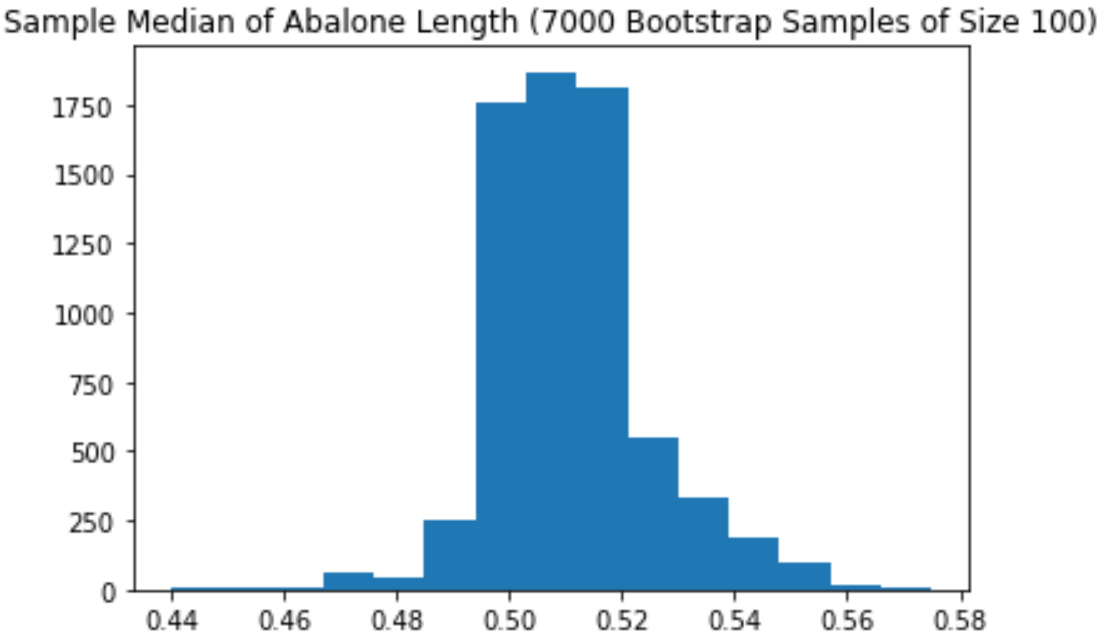
\includegraphics{HW7_1.PNG}
 
 \textbf{Part B: | Draw 10,000 samples of 30 records at random with replacement. Use each sample to produce a bootstrap estimate of a centered 90\% confidence interval for the population median. For what fraction of samples does the true population median lie inside the interval?}\newline
 
 Fraction of samples for which true population median lies inside interval: $0.875$
 
 \textbf{Part C: | Draw 10,000 samples of 10 records at random with replacement. Use each sample to produce a bootstrap estimate of a centered 90\% confidence interval for the population median. For what fraction of samples does the true population median lie inside the interval?}\newline
 
 Fraction of samples for which true population median lies inside interval: $0.825$
 
 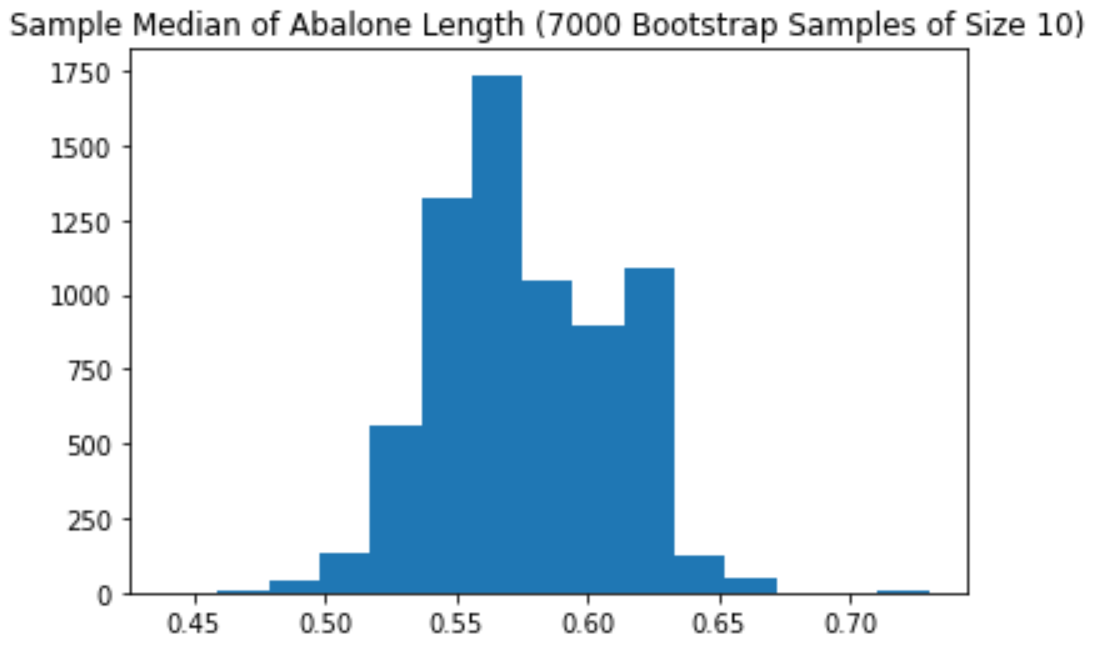
\includegraphics{HW7_2.PNG}
 
 \textbf{Part D: | What conclusion do you draw?}\newline
 
 It is pretty clear that the distribution in part C is more spread out than the distribution in part A. This is expected, because we used a much smaller sample size which may not be representative of the whole sample. Naturally, a smaller fraction of intervals in part C contained the population mean. Bootstrapping is not an end-all-be-all solution for small sample sizes, and it is important to understand that bootstrapping does not create new data.
 
 \newpage
 
 \noindent\makebox[\linewidth]{\rule{\paperwidth}{0.4pt}}\newline
 
 \begin{center}
      \Large\textbf{Problem 2:} In 1998, the average height of an adult male in South Africa was estimated to be 169 cm. Assume that this estimate is exact; assume also that the population standard deviation is 10 cm. What fraction of samples consisting of 50 adult males from South Africa (selected uniformly at random, and with replacement) will have average height greater than 200 cm?\par
 \end{center}
 
 We can use z-Scores and the sample mean distribution to solve this problem. We know that the standard deviation of the sample mean distribution, otherwise known as the standard error, is calculated using the following formula: $SE=\frac{\sigma}{\sqrt{N}}$, where $\sigma$ is the population standard deviation and $n$ is the sample size. The mean of the sample mean distribution is, of course, $169$ cm - unchanged from the population mean. 
 
 \[SE=\frac{\sigma}{\sqrt{N}}=\frac{10}{\sqrt{50}}=1.414\]
 
 We must calculate the z-score of $200$ cm. We will use $SE$ as the standard deviation.
 
 \[z = \frac{\hat{x} - \bar{x}}{s} = \frac{200-169}{1.414} = 21.924\]
 
 Using a z-score table, we find that $100 \%$ of values have a lower z-score, meaning that $0$ values have a higher z-score. This means that there is a $0 \%$ chance that a sample of 50 people will have a mean height greater tham $200$ cm. Of course, there is a negligible percentage of samples which will have a mean height of over $200$ cm, but that number is statistically insignificant.
 
 Final Answer: $0 \%$.\newline
 
 \newpage

 \begin{center}
      \Large\textbf{Problem 3:} Assume the average weight of an adult male short-hair house cat is 5 kg, and the standard deviation is 0.7 kg (these numbers are reasonable, but there’s quite a lively fight between cat fanciers about the true numbers).
      \par
 \end{center}

 \textbf{Part A: | What fraction of samples consisting of 30 adult male short-hair house cats (selected uniformly at random, and with replacement) will have average weight less than 4 kg?}\newline
 
 Once again, we must use z-scores and the distribution of sample means.
 
 \[SE=\frac{\sigma}{\sqrt{N}}=\frac{0.7}{\sqrt{30}}=0.128\]
 
 \[z = \frac{\hat{x} - \bar{x}}{s} = z = \frac{4-5}{0.128}=-7.813\]
 
 \[p = \int_{-\infty}^{7.813}\frac{1}{\sqrt{2\pi}}exp(\frac{-x^2}{2})dx = 2.8 * 10^{-15} \approx 0\]
 
 Using the z-score table, we find that effectively $0 \%$ of samples of size 30 have a mean weight less than 4kg. The z-score is so far from 0 (on the negative side) that virtually no values lie to the left on the distribution. The p-value is so negligible that we can approximate it to be 0.
 
 \textbf{Part B: | What fraction of samples consisting of 300 adult male short-hair house cats (selected uniformly at random, and with replacement) will have average weight less than 4 kg?}\newline
 
 Once again, we must use z-scores and the distribution of sample means.
 
 \[SE=\frac{\sigma}{\sqrt{N}}=\frac{0.7}{\sqrt{300}}=0.0404\]
 
 \[z = \frac{\hat{x} - \bar{x}}{s} = z = \frac{4-5}{0.0404}=-24.752\]
 
 \[p = \int_{-\infty}^{-24.813}\frac{1}{\sqrt{2\pi}}exp(\frac{-x^2}{2})dx = \approx 0\]
 
 Using the z-score table, we find that effectively $0 \%$ of samples of size 300 have a mean weight less than 4kg. The z-score is so far from 0 (on the negative side) that virtually no values lie to the left on the distribution. The integral calculator itself returned 0, implying that the integral is extremely small.
 
 \textbf{Part C: | Why are these numbers different?}\newline
 
 Although the numbers are technically both 0, it is clear that percentage in part B is less than the percentage in part A when we look at the results of the integrals. Because we used a larger sample in part B, it makes our standard error much smaller (and thus, our prediction more accurate), we find that a lower fraction of samples in part B are less than 4 than in part A. 
 
 \newpage
 
 \noindent\makebox[\linewidth]{\rule{\paperwidth}{0.4pt}}\newline
 
 \begin{center}
      \Large\textbf{Problem 4:} The Parktown prawn is an impressively repellent large insect, common in Johannesburg (look them up on the Web). I claim that their average length is 10 cm. You collect 100 Parktown prawns (this will take about 10 mins, in the right places in Johannesburg; more difficult from the US). The mean length of these prawns is 7 cm. The standard deviation is 1 cm. Assess the evidence against my claim.\par
 \end{center}
 
 We will use a significance level equal to $0.05$ - a standard value used by many statisticians - in order to figure out whether we accept or reject the claim that the average length is 10 cm. The test must be two-tailed, since the sampling distribution is a full normal distribution in our problem. We will use the z-score (not the t-score, because our sample size is large).
 
 \[SE = \frac{s}{\sqrt{n}} = \frac{1}{\sqrt{100}} = 0.1\]

 \[z = \frac{\hat{x}-\bar{x}}{SE} = \frac{10-7}{0.1} = 30\]

 When using a z-score table, we quickly find that the z-score is so far from 0 (on the positive side) that our p-value is effectively 0 for a two-tailed hypothesis test. Because $p < 0.05$, we must reject the claim. 

 \newpage
 
 \noindent\makebox[\linewidth]{\rule{\paperwidth}{0.4pt}}\newline
 
 \begin{center}
     \Large\textbf{Problem 5:} equiprobable? In Carcelle-le-Grignon at the end of the eighteenth century, there were 2009 births. There were 983 boys and 1026 girls. You can regard this as a fair random sample (with replacement, though try not to think too hard about what that means) of births. Assess the evidence against the hypothesis that a boy is born with probability exactly 0.5.\par
 \end{center}
 
 We need to use z-scores and the distribution of sample proportions to assess the hypothesis. We will use an alpha of 0.05 (a common value) for our hypothesis test. We will use the alternative hypothesis $p != 0$ and the null hypothesis $p = 0.5$. Of course, we can reject the null hypothesis (the claim) only if $p \leq 0.05$.
 
 \[p = \frac{983}{983 + 1026} = 0.489\]
 
 \[SE = \sqrt{\frac{p(1-p)}{n}} = \sqrt{\frac{0.489(1-0.489)}{2009}} = 0.0112\]
 
 \[z = \frac{\hat{p} - p}{SE} = \frac{0.489 - 0.5}{0.0112} = -0.982\].
 
 Using a two-tailed hypothesis test, we find the p-value to be 0.326 using a p-value table. Obviously, $p \geq 0.05$, and cannot reject the null hypothesis that the probability that a person is born male is 0.5.

 \end{document}

